\section{PAMS Architecture}\label{sec:arch}

This section develops \PAMS{} in three layers. \Cref{sec:math} derives the decision predicate and proves it exact. \Cref{sec:rtl} shows how the final RTL, \file{final/rtl/pams\_jqr.v}, computes each term. \Cref{sec:circuit} follows the RTL into synthesized gates and the placed-and-routed layout.

The design evaluated throughout is \sig{pams\_jqr}. It is the frozen \PAMS{} algorithm of the original design \sig{pams} with three implementation-level changes, none of which changes the decision function:
\begin{itemize}
  \item just-in-time operand delays;
  \item a two-stage share-wise multiplier;
  \item retimed public logic.
\end{itemize}

\subsection{Mathematical Construction}\label{sec:math}

\paragraph{A.~The exact problem.}
One coefficient is verified per clock cycle. The circuit receives:
\begin{itemize}
  \item three \emph{canonical} arithmetic shares $x_0, x_1, x_2 \in \{0, \dots, q-1\}$ of the re-encrypted coefficient $x = x_0 + x_1 + x_2 \bmod q$;
  \item the public received compressed coefficient $c \in [0, 2^d)$;
  \item the public width $d \in \{4, 5, 10, 11\}$.
\end{itemize}
It must output a three-share Boolean sharing of
\begin{equation}\label{eq:target}
  b \;=\; \bigl[\, \Comp(x) = c \,\bigr] \in \{0,1\},
\end{equation}
and, over a ciphertext, a sharing of $D = \bigwedge b$ (\cref{eq:pred}). Neither $x$ nor $b$ may be recombined.

A direct approach computes a masked $\Comp(x)$ (a $d$-bit Boolean sharing) and then tests equality with $c$. In hardware the masked compression is itself a modulus switch plus a Boolean adder whose width grows with $d$, as in Simple and HOCompress. The equality is a further $d$-bit zero test. \PAMS{} never forms $\Comp(x)$. It asks directly whether $x$ lies in the public interval $I_c$, and it formulates that question so that the protected adder has the same small width for every $d$.

\paragraph{B.~Notation.} The following symbols are used throughout the paper.
\begin{center}\footnotesize
\begin{tabularx}{\columnwidth}{@{}>{\raggedright\arraybackslash}p{3.0cm}X@{}}
\toprule
symbol & meaning \\
\midrule
$q = 3329$, $n = 3$ & modulus; number of shares \\
$d \in \{4,5,10,11\}$ & compression width (per coefficient) \\
$x_i$, $x$ & canonical shares; $x = \sum x_i \bmod q$ \\
$c \in [0, 2^d)$ & public compressed coefficient \\
$K = 14$ & width of the switched representation \\
$F_K(v) = \lfloor 2^K v / q \rfloor$ & modulus switch (any integer $v$) \\
$y_i = F_K(x_i)$ & switched share $i$ (secret, domain $i$) \\
$j \in \{0,1,2\}$ & integer switching error, \cref{eq:lemma} \\
$a_c$; $I_c = [a_c, a_{c+1})$ & public interval of $c$, \cref{eq:interval} \\
$\Low_c = F_K(a_c) \bmod 2^K$ & public anchor \\
$\Theta_c$ & public threshold, \cref{eq:theta} \\
$\hat y_0 = y_0 + 2 - \Low_c$ & anchored share 0 (mod $2^K$) \\
$Z = \hat y_0 + y_1 + y_2$ & masked switched offset (mod $2^K$) \\
$b = [Z < \Theta_c]$ & per-coefficient decision \\
$g$ & minimum gap of $F_K$, \cref{eq:gap} \\
\bottomrule
\end{tabularx}
\end{center}
All arithmetic on $y_i$, $\Low_c$, $\Theta_c$ and $Z$ is modulo $2^K$, i.e.\ on 14-bit words.

\paragraph{C.~Share-wise modulus switching.}
A power-of-two modulus is what hardware adds natively: a $K$-bit adder computes sums mod $2^K$ by discarding the carry out. Mod $q$, by contrast, needs a comparison and a conditional subtraction. Masked Boolean addition is the expensive part of every exact comparison, so we want it to happen mod $2^K$ with small $K$.

The map $F_K$ is applied to each share separately. This is share-local: domain $i$ computes $y_i = F_K(x_i)$ from its own share with a constant multiplier, and no other domain is involved. The sum of the switched shares is close to the switched secret.
\begin{lemma}[integer-error switching; Coron et al.~\cite{coron2023dil}, Lemma~2]\label{lem:switch}
For canonical shares $x_0, \dots, x_{n-1} \in [0, q)$ with $x = \sum x_i \bmod q$,
\begin{equation}\label{eq:lemma}
  \sum_{i} F_K(x_i) \;\equiv\; F_K(x) - j \pmod{2^K}
\end{equation}
for some integer $j \in \{0, 1, \dots, n-1\}$.
\end{lemma}
\begin{proof}
\emph{Step 1 (one share).} Write $2^K x_i = q F_K(x_i) + r_i$ with remainder $r_i \in [0, q)$. Summing over $i$,
\[ q \textstyle\sum_i F_K(x_i) = 2^K \sum_i x_i - \sum_i r_i . \]

\emph{Step 2 (the secret).} Since $\sum_i x_i = x + kq$ with $k \in \{0, \dots, n-1\}$ and $2^K x = q F_K(x) + r$ with $r \in [0, q)$, we have
\[ q \textstyle\sum_i F_K(x_i) = q F_K(x) + r + 2^K k q - \sum_i r_i . \]

\emph{Step 3 (remainders).} Reducing mod $q$ shows $\sum_i r_i \equiv r \pmod q$. Because $0 \le \sum_i r_i \le n(q-1)$, we get $\sum_i r_i = r + jq$ for an integer $j$ with $0 \le j \le n - 1$.

\emph{Step 4.} Substituting and dividing by $q$ gives $\sum_i F_K(x_i) = F_K(x) - j + 2^K k$, which is \cref{eq:lemma}.
\end{proof}
The error $j$ is secret and unknown. It depends on the shares, not only on $x$. For $K = 14$, $j = 2$ occurs for 3,327 of the 3,329 values of $x$; Phase XII enumerated all $3329^3 = \num{36892780289}$ canonical triples with 0 violations. \PAMS{} absorbs the error by a public offset of $n - 1 = 2$ (the same offset as ModSwitch~\cite{coron2023dil}): $\sum F_K(x_i) + 2 = F_K(x) + (2 - j)$ with $2 - j \in [0, 2]$. The decision is then chosen so that an error in $[0, 2]$ can never move a value across a decision boundary.

\paragraph{D.~Interval anchors and thresholds.}
By \cref{eq:interval}, $b = 1$ iff $x \in [a_c, a_{c+1})$ cyclically. Rather than testing two bounds, \PAMS{} moves the interval start to zero. The anchor $\Low_c = F_K(a_c)$ is subtracted, and the interval end becomes the single public threshold
\begin{equation}\label{eq:theta}
  \Theta_c \;=\; F_K(a_{c+1}) - F_K(a_c) - 1 \pmod{2^K}.
\end{equation}
Both depend only on the public pair $(c, d)$. The RTL evaluates them through closed forms. With $e = 13 - d$, $r_c = ((1 - 2c)\,q) \bmod 2^{d+1}$ and $\mathrm{qq}(r) = \lfloor r\,2^{e}/q \rfloor \in [0, 4]$ (derived in \cref{app:math-anchors}):
\begin{align}
  \Low_c &= (2c - 1)\, 2^{e} + \mathrm{qq}(r_c) \pmod{2^{14}}, \label{eq:low}\\
  \Theta_c &= 2^{e+1} - 1 + \mathrm{qq}(r_{c+1}) - \mathrm{qq}(r_c), \label{eq:thetaclosed}
\end{align}
where $r_{c+1} = (r_c - 2q) \bmod 2^{d+1}$.
Over all 3,120 pairs $(c, d)$, $3 \le \Theta_c \le 1027 < 2^{11}$.

\emph{Wraparound.} The interval $I_0$ wraps through $q - 1 \to 0$; for $d = 4$, $a_0 = 3225$ and $a_1 = 105$. Arithmetic mod $2^K$ handles this without a special case. $F_K$ satisfies $F_K(v + q) = F_K(v) + 2^K$, so the switched positions of $\Zq$ lie on a circle of circumference $2^K$, just as $\Zq$ itself is a circle of circumference $q$. Subtracting $\Low_c$ mod $2^K$ rotates that circle so that $I_c$ starts at 0.

\paragraph{E.~The complete predicate.} From arithmetic shares to the protected decision:
\begin{align}
  y_i &= F_K(x_i) = (x_i \cdot 10321339) \gg 21 , \label{eq:yi}\\
  \hat y_0 &= y_0 + 2 - \Low_c \bmod 2^{14} , \label{eq:y0}\\
  Z &= \hat y_0 + y_1 + y_2 \bmod 2^{14} , \label{eq:Z}\\
  b &= [\, Z < \Theta_c \,] . \label{eq:b}
\end{align}
\Cref{eq:yi} is computed share-wise on secret data. \Cref{eq:y0} touches share 0 only and adds the public $\Low_c$. \Cref{eq:Z} is the masked three-operand sum, and \cref{eq:b} the masked comparison with the public $\Theta_c$.
The multiplier constant $M = 10321339$ and shift $21$ give $\lfloor x_i 2^{14}/q \rfloor$ exactly for every $x_i \in [0, q)$ (Phase XII check B).

\emph{Public versus secret terms.}
\begin{itemize}
  \item \emph{Public:} $\Low_c$, $\Theta_c$ and every bit of them.
  \item \emph{Secret:} each $y_i$ is known only to domain $i$, and no domain ever holds $Z$, $j$ or $b$ in the clear.
  \item \emph{Where the sharing is converted:} \cref{eq:Z,eq:b} are evaluated on a Boolean sharing in which $y_i$ is share $i$ and the other two shares are zero. A carry-save adder (CSA) reduces the three operands to two. A ripple carry chain then computes $Z$ bit by bit, and a ripple comparator against the public bits of $\Theta_c$ runs alongside it.
\end{itemize}
Because $\Theta_c$ is public, each comparator step costs one AND gadget, and all negations of $\Theta_c$ bits are applied to share 0 for free. Because $\Theta_c < 2^{11}$, the comparator splits: $b = [Z_{13:11} = 0] \wedge [Z_{10:0} < \Theta_{c,10:0}]$. The top three bits need only a carry-free zero test. \Cref{tab:kernel} lists the resulting gadget budget next to the Simple baseline.

\begin{table}[t]\centering\small
\caption{HPC2 gadgets per lane by function (counted in the RTL; identical in every mapped netlist).}\label{tab:kernel}
\begin{tabular}{@{}lrr@{}}
\toprule
part & \PAMS{} & Simple baseline \\
\midrule
CSA majorities (3 operands $\to$ 2) & 13 & 23 \\
ripple carries & 10 & 12 \\
comparator against $\Theta_c$ & 10 & -- \\
top region (zero test, OR tree) & 4 & 20 \\
final combination & 1 & 0 \\
ciphertext accumulator & 2 & 2 \\
\midrule
\textbf{total} & \textbf{40} & \textbf{57} \\
fresh random bits per cycle ($3 \times$) & 120 & 171 \\
masked operand width & 14 bit & 24 bit \\
\bottomrule
\end{tabular}
\end{table}

\paragraph{F.~Exactness.}\label{sec:exact}
The proof uses one property of $F_K$: consecutive switched values are at least $g$ apart, where
\begin{equation}\label{eq:gap}
  g \;=\; \min_{v \in \Z}\bigl(F_K(v+1) - F_K(v)\bigr) = \lfloor 2^K/q \rfloor .
\end{equation}
For $K = 14$, $2^{14}/q = 4.92$, so $g = 4$ and every step of $F_{14}$ is 4 or 5. This holds also across the wrap, since $2^{14} - F_{14}(q-1) = 5$. For $K = 13$, $g = 2$.

\begin{proposition}[exactness of \PAMS{}]\label{prop:exact}
Let $K = 14$, $d \in \{4,5,10,11\}$, $c \in [0, 2^d)$ and canonical shares $x_0, x_1, x_2 \in [0, q)$ of $x$. Define $Z$ by \cref{eq:yi,eq:y0,eq:Z} and $\Theta_c$ by \cref{eq:theta}. Then $[Z < \Theta_c] = [\Comp(x) = c]$. More precisely, members satisfy $0 \le Z \le \Theta_c - 1$, and non-members satisfy $\Theta_c + 1 \le Z \le 2^{14} - 2$.
\end{proposition}
\begin{proof}
\emph{Setup.} By \cref{lem:switch}, $Z \equiv F_K(x) - F_K(a_c) + (2 - j) \pmod{2^K}$ with $2 - j \in [0, 2]$.
\begin{itemize}
  \item Let $\tilde x$ be the representative of $x$ in $[a_c, a_c + q)$ and $\tilde a$ that of $a_{c+1}$ in $(a_c, a_c + q]$.
  \item Quasi-periodicity gives $F_K(\tilde x) \equiv F_K(x)$, so $Z \equiv \Delta + (2 - j)$ with $\Delta = F_K(\tilde x) - F_K(a_c) \in [0, 2^K)$.
  \item Put $D_c = F_K(\tilde a) - F_K(a_c)$. Since $0 < D_c < 2^K$, $\Theta_c = D_c - 1$ as an integer.
\end{itemize}

\emph{Members} ($a_c \le \tilde x \le \tilde a - 1$). Here $0 \le \Delta \le F_K(\tilde a - 1) - F_K(a_c) \le D_c - g$, so $0 \le \Delta + 2 - j \le D_c - g + 2 = \Theta_c + 3 - g$. With $g = 4$ this is at most $\Theta_c - 1 < 2^K$: no wrap occurs, and $Z < \Theta_c$.

\emph{Non-members} ($\tilde a \le \tilde x \le a_c + q - 1$). Here $\Delta \ge D_c$, and $\Delta \le F_K(a_c + q - 1) - F_K(a_c) \le 2^K - g$. Hence $\Theta_c + 1 = D_c \le \Delta + 2 - j \le 2^K - g + 2 = 2^K - 2$. Again no wrap occurs, and $Z \ge \Theta_c$.
\end{proof}
The bounds are tight. Evaluating every $(x, j, c, d)$ for this paper gives $\max(Z - \Theta_c) = -1$ over members and $\min(Z - \Theta_c) = +1$ over non-members. Phase XII's exhaustive check of the decision rule over all $3329 \cdot 3 \cdot (2^4 + 2^5 + 2^{10} + 2^{11})$ cases found 0 mismatches. Together with \cref{lem:switch}, that enumeration is a second, computational proof for the stated input contract, assuming the enumeration script is correct (\cref{app:math-exact}). This review re-ran the bound check (\file{paper/scripts/audit\_math.py}), but did not repeat the $3329^3$ lemma enumeration.

\begin{remark}[scope of the 14-bit requirement]\label{rem:k13}
The proof needs $g \ge 4$ for the chosen offset and threshold. Any exact rule on $Z$ needs $g \ge 3$, because an error range of width 3 must fit between neighbouring switched values. The first $K$ with $\lfloor 2^K/q \rfloor \ge 3$ is $K = 14$. At $K = 13$ ($g = 2$), members and non-members collide on \emph{reachable} share triples for every $d$. For example, at $d = 11$, $x = 0$ shared as $(0, 0, 0)$ and $x = 1$ shared as $(3326, 2, 2)$ give the same switched sum. So no decision function of $Z$ can be exact.

This lower bound holds \emph{only in the share-wise floor model}, where $y_i = \lfloor 2^K x_i/q \rfloor$ and the decision depends only on $\sum y_i$ plus public offsets. It is not a lower bound for all masked circuits: other conversions (prime-modulus A2B, rounding with share-dependent offsets) are outside it.
\end{remark}

\emph{Canonical shares.} The proof is stated for canonical shares $x_i < q$, and the hardware is verified only for them. Two facts bound what happens outside that range.
\begin{itemize}
  \item The proof of \cref{lem:switch} does not itself use $x_i < q$: it holds for any non-negative integer shares.
  \item The 12-bit constant multiplier equals $F_{14}$ (mod $2^{14}$) on every 12-bit input except $x_i = 3329$ and $x_i = 4005$, where it is one too small.
\end{itemize}
Our review searched non-canonical inputs only by sampling and found no wrong decision, but it did not analyse them completely. Such inputs would affect correctness, not masking. Neither \PAMS{} nor the baseline checks its inputs, so canonical shares are an interface requirement on the upstream masked re-encryption, for both designs alike.

\paragraph{G.~Worked examples.} \Cref{tab:examples} traces four coefficients through \cref{eq:yi,eq:y0,eq:Z,eq:b}.
\begin{itemize}
  \item \textbf{Source:} every value was computed by the reference model (\file{models/pams.py}). It was then \emph{independently} read back from the internal registers of the simulated final RTL (\file{paper/scripts/examples.py}); the two agree exactly.
  \item \textbf{E1} is a member of the wrapped interval $I_0$ at $d = 4$.
  \item \textbf{E2} is the first value of the next interval at $d = 11$, with the worst-case error $j = 2$. It is rejected with the minimum possible margin, $Z = \Theta_c + 1$.
  \item \textbf{E3} is the last member of its interval at $d = 10$.
  \item \textbf{E4} lies just before the start of $I_0$ and wraps to $Z = 2^{14} - 5$.
\end{itemize}

\begin{table*}[t]\centering\small
\caption{Worked examples (all values mod $2^{14}$ unless stated). Shares and every intermediate quantity were verified against the internal registers of the simulated \sig{pams\_jqr} RTL: \sig{x$i$r}, \sig{s$i$p} ($=y_i$), \sig{y0} ($=\hat y_0$), \sig{lowp} ($=\Low_c$), \sig{th2} ($=\Theta_c$), and the recombined \sig{cdec} at stage~31.}\label{tab:examples}
\setlength{\tabcolsep}{3pt}
\resizebox{\textwidth}{!}{%
\begin{tabular}{@{}lrrrrrrrrrrrrrr@{}}
\toprule
 & $x$ & $(x_0, x_1, x_2)$ & $d$ & $c$ & $\Comp(x)$ & $[a_c, a_{c+1})$ & $F_{14}(x)$ & $(y_0, y_1, y_2)$ & $j$ & $\Low_c$ & $\Theta_c$ & $\hat y_0$ & $Z$ & $b$ \\
\midrule
E1 & 3300 & (487, 1308, 1505) & 4 & 0 & 0 & [3225, 105) & 16241 & (2396, 6437, 7407) & 1 & 15872 & 1027 & 2910 & 370 & 1 \\
E2 & 1627 & (1722, 3208, 26) & 11 & 1000 & 1001 & [1625, 1627) & 8007 & (8474, 15788, 127) & 2 & 7997 & 9 & 479 & 10 & 0 \\
E3 & 976 & (2345, 2243, 3046) & 10 & 300 & 300 & [974, 977) & 4803 & (11541, 11039, 14991) & 0 & 4793 & 14 & 6750 & 12 & 1 \\
E4 & 3224 & (3076, 3166, 311) & 4 & 0 & 15 & [3225, 105) & 15867 & (15138, 15581, 1530) & 2 & 15872 & 1027 & 15652 & 16379 & 0 \\
\bottomrule
\end{tabular}}
\end{table*}

For E1, step by step:
\begin{itemize}
  \item Share-wise switching gives $y = (2396, 6437, 7407)$, whose sum is $16240 \equiv F_{14}(3300) - 1$. Hence $j = 1$.
  \item Share 0 is anchored to $\hat y_0 = 2396 + 2 - 15872 \equiv 2910$.
  \item The masked sum is $Z = 2910 + 6437 + 7407 = 16754 \equiv 370$.
  \item $370 < \Theta_0 = 1027$, so $b = 1$, and indeed $\Comp(3300) = 0$.
\end{itemize}
In E4 the switched sum lands just \emph{below} the anchor. The subtraction wraps to $Z = 16379$, far above $\Theta_0$, which is the cyclic behaviour that removes any special case for $I_0$. \Cref{fig:boundaries} plots $Z$ against $x$ at both ends of $I_0$ for all three values of $j$.

\begin{figure*}[t]\centering
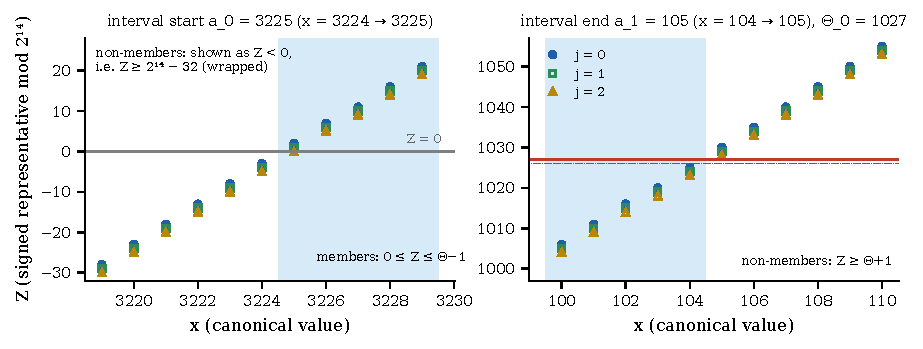
\includegraphics[width=\textwidth]{figures/mathematics/fig_switch_boundaries.pdf}
\caption{$Z$ as a function of the canonical value $x$ near both ends of the wrapped interval $I_0$ ($d = 4$, $\Theta_0 = 1027$), for the three possible switching errors $j$. Members are shaded.
\emph{Left:} at the interval start, members begin at $Z \in [0, 2]$, and non-members just below $a_0$ wrap to $Z \ge 2^{14} - 32$, drawn as negative values.
\emph{Right:} at the interval end, the last member reaches at most $\Theta_0 - 1$ (dotted) and the first non-member at least $\Theta_0 + 1$.
Generated from \file{models/pams.py} by \file{paper/scripts/generate\_figures.py}.}\label{fig:boundaries}
\end{figure*}

\paragraph{H.~From equations to hardware.} \Cref{tab:map} names the RTL signals that compute each quantity. It also gives the pipeline stage at which each value is held, where stage $s$ means $s$ clock edges after the coefficient enters. A full cross-layer map, including gate-level regions and figure references, is in \cref{app:traceability} and \file{paper/CROSS\_LAYER\_TRACEABILITY.md}.

\begin{table*}[t]\centering\small
\caption{Mathematical quantities and the \sig{pams\_jqr} RTL that computes them (stage = register boundary at which the value is held).}\label{tab:map}
\setlength{\tabcolsep}{4pt}
\begin{tabularx}{\textwidth}{@{}p{3.4cm}Xp{6.4cm}@{}}
\toprule
quantity & hardware representation & RTL (stage) \\
\midrule
$x_i$ & 12-bit input, then two register stages & \sig{x$i$}, \sig{x$i$q} (1), \sig{x$i$r} (2) \\
$F_{14}(x_i)$ & $(x_i \cdot M) \gg 21$; two registered partial products, then sum & \sig{mh$i$}, \sig{ml$i$} (3), \sig{s$i$p} (4) \\
$e$, $\mathrm{qq}(r_c)$, $\mathrm{qq}(r_{c+1})$ & public logic from $(c, d)$ & \sig{e0r}, \sig{qcr}, \sig{qnr} (2) \\
$\Low_c$, $\Theta_c$ & \cref{eq:low,eq:thetaclosed} & \sig{lowrq}, \sig{thrq} (3), \sig{lowp} (4), \sig{th2} (5) \\
$\hat y_0, y_1, y_2$ & 14-bit operands, one per domain & \sig{y0}, \sig{y1}, \sig{y2} (5) \\
$Z$, $[Z < \Theta_c]$ & CSA + ripple carry + comparator: 38 HPC2, share-local XOR, delay registers & \sig{ug111}\ldots\sig{ug1542}, \sig{r105}\ldots (5--31) \\
$b$ (3 shares) & Boolean sharing & \sig{cdec}, \sig{cvalid} (31) \\
$D$ (3 shares) & AND accumulator over the ciphertext & \sig{uacc}, \sig{ufin}, \sig{dec}, \sig{dvalid} (35) \\
\bottomrule
\end{tabularx}
\end{table*}

\subsection{Verilog Implementation}\label{sec:rtl}
The final RTL is generated by \file{competitors/models/cgen.py} from the same building blocks as the frozen generator \file{models/gen.py}. With all optimizations disabled, the generator reproduces the frozen \file{rtl/pams.v} byte for byte. \file{final/rtl/pams\_jqr.v} has 2,747 lines.
\begin{itemize}
  \item Lines 1--19: the HPC2 module.
  \item Lines 21--56: the lane interface, input registers, public window logic and share-wise front end.
  \item Lines 58--1499: generated wire and register declarations.
  \item Lines 1500--1537: the 38 kernel gadget instances.
  \item Lines 1538--2729: share-local delay registers.
  \item Lines 2730--2746: the control pipeline and the accumulator.
\end{itemize}
All excerpts below are verbatim, with their source line numbers. \Cref{app:verilog} explains the remaining code.

\paragraph{Interface and input registers (lines 21--26).}\leavevmode\par
\lstinputlisting[firstline=21,lastline=26,firstnumber=21]{\RTL}
\begin{itemize}
  \item \textbf{Ports.} The three 12-bit shares arrive on \sig{x0..x2}, the public \sig{c} and \sig{mode} beside them, and \sig{vin}/\sig{first}/\sig{last} frame a ciphertext. The 120-bit port \sig{rnd} carries the fresh randomness of the cycle: 3 bits for each of the 40 gadgets.
  \item \textbf{Stage 1.} All inputs are registered; \sig{mode} is decoded to $d$ in \sig{d0}.
  \item \textbf{Domains.} The share index is kept in the signal names (\sig{x0q}, \sig{x1q}, \sig{x2q}), which is how the structural checks of \cref{sec:security} identify domains. Nothing ever combines two of these signals outside a gadget.
\end{itemize}

\paragraph{Public anchor and threshold (lines 31--45).}\leavevmode\par
\lstinputlisting[firstline=31,lastline=45,firstnumber=31]{\RTL}
\begin{itemize}
  \item \textbf{Closed forms.} This is \cref{eq:low,eq:thetaclosed}. \sig{qq} implements $\lfloor r\,2^{e}/q \rfloor$ with four constant comparisons (line~34), \sig{pr} is $(1 - 2c)\,q \bmod 2^{12}$ (line~38), and \sig{rmask} reduces it mod $2^{d+1}$.
  \item \textbf{Retiming (r).} The intermediate results \sig{qc}, \sig{qn}, \sig{e0} and \sig{c0} are registered at stage~2 (line~43). The remaining arithmetic producing \sig{lowr} = $\Low_c$ and \sig{thr} = $\Theta_c$ completes in the next stage (lines~44--45). This splits a public critical path (\cref{sec:circuit}) without adding latency.
  \item \textbf{Security.} Everything here is a function of public $(c, d)$ only.
\end{itemize}

\paragraph{Share-wise modulus switch (lines 47--56).}\leavevmode\par
\lstinputlisting[firstline=47,lastline=56,firstnumber=47]{\RTL}
\begin{itemize}
  \item \textbf{Partial products (stage 3, line~49).} Each share is split as $x_i = 2^6 x_{i,11:6} + x_{i,5:0}$, and both halves are multiplied by $M$ and registered. Line~49 is long because the generator emits all six products on one line.
  \item \textbf{Recombination (lines~50--51).} \sig{m$i$} recombines the halves, and \sig{s$i$} drops 21 bits to give $y_i = F_{14}(x_i)$ (\cref{eq:yi}), registered as \sig{s$i$p} at stage 4.
  \item \textbf{Anchoring (stage 5, line~56).} Share 0 receives $-\Low_c + 2$ (\cref{eq:y0}). Shares 1 and 2 pass unchanged. The public threshold is delayed alongside the data into \sig{th2}.
  \item \textbf{Locality.} Each multiplier sees one share only. The 14-bit outputs \sig{y0..y2} are the only secret inputs of the masked kernel.
\end{itemize}

\paragraph{Masked kernel: gadget instances and delay registers.}
The kernel is generated as flat wires, registers and \sig{hpc2} instances. Its first three gadgets implement bit 1 of the adder and comparator:
\lstinputlisting[firstline=1500,lastline=1502,firstnumber=1500]{\RTL}
\begin{itemize}
  \item \textbf{\sig{ug111}: CSA majority of bit 0, $T_1 = \mathrm{maj}(y_{0,0}, y_{1,0}, y_{2,0})$.} It uses $\mathrm{maj}(a, b, c) = ((a \oplus b) \wedge (a \oplus c)) \oplus a$. Its operand sharings $(y_{0,0}, y_{1,0}, 0)$ and $(y_{0,0}, 0, y_{2,0})$ are formed from the three single-domain bits without any XOR gate, because the third share is the constant 0.
  \item \textbf{\sig{ug134}: carry $c_2 = S_1 \wedge T_1$.} Here $S_1$ is held as three single-domain registered bits \sig{r106}, \sig{r108}, \sig{r110}.
  \item \textbf{\sig{ug128}: comparator step for bit 1.} It computes $\lt_2 = ((z_1 \oplus \bar\theta_1) \wedge (\lt_1 \oplus \theta_1)) \oplus \theta_1$, with $z_1 = S_1 \oplus T_1$ and the public $\theta_1$ applied to share 0.
  \item \textbf{Randomness.} Each instance takes its own 3-bit slice of \sig{rnd}.
\end{itemize}

The delay registers that align operands are plain share-local shift registers, for example
\lstinputlisting[firstline=1538,lastline=1548,firstnumber=1538]{\RTL}
Bit $k$ of each operand waits until the carry for bit $k$ arrives, about $2k$ cycles later. Each chain holds one share bit, so the registers never mix domains.

\paragraph{Control and accumulation (lines 2730--2746).}\leavevmode\par
\lstinputlisting[firstline=2730,lastline=2746,firstnumber=2730]{\RTL}
\begin{itemize}
  \item \textbf{Control.} \sig{vp}, \sig{fp} and \sig{lp} delay the public frame signals to stage 31, where \sig{cdec} (the output of \sig{ug1542}) is the per-coefficient decision.
  \item \textbf{Accumulator.} \sig{uacc} ANDs each decision into a running product. Its 2-cycle latency yields two interleaved chains (even and odd coefficients), which \sig{init\_p} starts at the first two coefficients of a ciphertext. \sig{ufin} ANDs the two chains into \sig{dec}, valid with \sig{dvalid} four cycles after the last coefficient's decision.
  \item \textbf{Throughput.} A new coefficient can enter every cycle (initiation interval 1). The ciphertext decision appears 35 cycles after its last coefficient entered, against 37 cycles for the baseline \sig{base\_jq}.
\end{itemize}

\subsection{Circuit Architecture and Physical Realization}\label{sec:circuit}

\begin{figure*}[t]\centering
\resizebox{\textwidth}{!}{% PAMS datapath (pams_jqr). Conceptual diagram reconstructed by hand from final/rtl/pams_jqr.v (signal names, widths
% and stages from the source; see FIGURE_PROVENANCE.md). Not an automatically extracted circuit.
\begin{tikzpicture}[x=1cm,y=1cm,font=\scriptsize,>={Stealth[length=1.6mm]},
  reg/.style={draw,fill=white,minimum width=1.0cm,minimum height=0.46cm,inner sep=1.5pt,align=center},
  op/.style={draw,rounded corners=2pt,fill=#1,minimum height=0.46cm,inner sep=2pt,align=center},
  op/.default=blue!8,
  lab/.style={font=\tiny,inner sep=1pt}]
  % stage guides
  \foreach \s/\x in {1/1.55,2/3.05,3/4.75,4/6.55,5/8.25} {
    \draw[gray!40,dashed] (\x,-3.4) -- (\x,1.2);
    \node[gray,font=\tiny] at (\x,1.45) {stage \s};
  }
  \node[gray,font=\tiny] at (11.75,1.45) {stages 5--31 (13 gadget levels $\times$ 2 cycles)};
  \node[gray,font=\tiny] at (15.0,1.45) {stage 31};
  \node[gray,font=\tiny] at (17.1,1.45) {stage 35};
  % share lanes; share 0 is drawn next to the public lane so that the Low_c arrow crosses no other lane
  \foreach \i/\y in {2/0.6,1/-0.2,0/-1.0} {
    \node[lab,anchor=east] at (0.45,\y) {$x_{\i}$ [11:0]};
    \node[reg] (q\i) at (1.55,\y) {\sig{x\i q}};
    \node[reg] (r\i) at (3.05,\y) {\sig{x\i r}};
    \node[op] (m\i) at (4.75,\y) {$\times M$ (split)\\[-1pt]\sig{mh\i}, \sig{ml\i}};
    \node[op] (s\i) at (6.55,\y) {$\gg 21$\\[-1pt]\sig{s\i p} [13:0]};
    \draw[->] (0.5,\y) -- (q\i); \draw[->] (q\i) -- (r\i); \draw[->] (r\i) -- (m\i); \draw[->] (m\i) -- (s\i);
  }
  \node[op=orange!12] (y0) at (8.25,-1.0) {$+2-\mathrm{Low}_c$\\[-1pt]\sig{y0} [13:0]};
  \node[reg] (y1) at (8.25,-0.2) {\sig{y1} [13:0]};
  \node[reg] (y2) at (8.25,0.6) {\sig{y2} [13:0]};
  \draw[->] (s0) -- (y0); \draw[->] (s1) -- (y1); \draw[->] (s2) -- (y2);
  % public lane
  \node[lab,anchor=east] at (0.45,-2.6) {$c$ [10:0], mode};
  \node[reg] (c0) at (1.55,-2.6) {\sig{c0}, \sig{d0}};
  \node[op=gray!12] (pw) at (3.05,-2.6) {$e$, $\mathrm{qq}(r_c)$,\\[-1pt]$\mathrm{qq}(r_{c+1})$};
  \node[op=gray!12] (lo) at (4.75,-2.6) {$\mathrm{Low}_c$, $\Theta_c$\\[-1pt]\sig{lowrq}, \sig{thrq}};
  \node[reg] (lp) at (6.55,-2.6) {\sig{lowp}, \sig{thp}};
  \node[reg] (th) at (8.25,-2.6) {\sig{th2} [13:0]};
  \draw[->] (0.5,-2.6) -- (c0); \draw[->] (c0) -- (pw); \draw[->] (pw) -- (lo); \draw[->] (lo) -- (lp); \draw[->] (lp) -- (th);
  \draw[->,gray] (lp.north east) -- node[lab,pos=0.45,right] {$\mathrm{Low}_c$} (y0.south west);
  % masked kernel
  \node[draw,thick,fill=orange!6,rounded corners=3pt,minimum width=4.7cm,minimum height=4.3cm] (k) at (11.75,-1.15) {};
  \node[font=\scriptsize\bfseries] at (11.75,0.72) {masked kernel: 38 HPC2};
  \foreach \t/\y in {{CSA: 13 maj (HPC2) $\to S, T$}/0.2, {ripple carry $c_2 \ldots c_{11}$: 10 HPC2}/-0.45,
                    {comparator vs.\ $\Theta_c$: 10 HPC2}/-1.1,
                    {zero test $Z_{13:11}$: 4 HPC2}/-1.75, {final AND $\to b$: 1 HPC2}/-2.4}
    \node[op=orange!22,minimum width=4.3cm] at (11.75,\y) {\t};
  \node[lab,align=center] at (11.75,-2.88) {+ share-local XORs and single-domain\\ delay registers};
  \draw[->] (y2.east) -- (9.4,0.6); \draw[->] (y1.east) -- (9.4,-0.2); \draw[->] (y0.east) -- (9.4,-1.0);
  \draw[->] (th.east) -- (9.4,-2.6);
  \node[lab,anchor=north] (rnd) at (11.75,-3.55) {\sig{rnd}[113:0]: 3 fresh bits per gadget};
  \draw[->,densely dotted] (rnd.north) -- (k.south);
  % output and accumulator
  \node[reg,minimum width=1.25cm] (cdec) at (15.0,-1.15) {\sig{cdec}[2:0]\\[-1pt]$b_0, b_1, b_2$};
  \draw[->] (k.east) -- (cdec);
  \node[op=orange!22,minimum width=2.0cm] (acc) at (17.1,-1.15) {\sig{uacc}, \sig{ufin}\\[-1pt]2 HPC2: $D = \wedge\, b$};
  \draw[->] (cdec) -- (acc);
  \node[lab] at (17.1,-1.85) {\sig{rnd}[119:114]};
  \node[reg,minimum width=1.1cm] (dec) at (17.1,0.35) {\sig{dec}[2:0]};
  \draw[->] (acc) -- (dec);
  \node[lab,align=center] at (15.4,-3.05) {\sig{cvalid}, \sig{dvalid}: from the\\ \sig{vin}/\sig{first}/\sig{last} pipeline};
  % legend
  \node[op,minimum height=0.22cm,minimum width=0.4cm] at (0.9,-3.75) {}; \node[lab,anchor=west] at (1.2,-3.75) {share-local logic (one domain)};
  \node[op=gray!12,minimum height=0.22cm,minimum width=0.4cm] at (0.9,-4.15) {}; \node[lab,anchor=west] at (1.2,-4.15) {public logic ($c$, $d$ only)};
  \node[op=orange!22,minimum height=0.22cm,minimum width=0.4cm] at (5.3,-3.75) {}; \node[lab,anchor=west] at (5.6,-3.75) {HPC2 gadgets (all three domains)};
  \node[reg,minimum height=0.22cm,minimum width=0.4cm] at (5.3,-4.15) {}; \node[lab,anchor=west] at (5.6,-4.15) {register stage};
\end{tikzpicture}
}
\caption{\PAMS{} datapath (\sig{pams\_jqr}). This is a conceptual diagram reconstructed from the RTL; widths and stage numbers are those of the source.
\textbf{Share lanes (blue):} each share is processed only within its own domain.
\textbf{Public lane (grey):} depends only on $(c, d)$.
\textbf{Masked kernel (orange):} the only place where domains meet, and only inside the 38 HPC2 gadgets. Each gadget takes 3 fresh bits from \sig{rnd}.
\textbf{Accumulator:} two further gadgets combine the per-coefficient decisions of a ciphertext.
Stage $s$ = number of clock edges after the coefficient enters.}\label{fig:datapath}
\end{figure*}

\paragraph{Architectural level.}
\Cref{fig:datapath} shows the complete datapath, organized as five stages of share-local front end followed by the masked kernel.
\begin{itemize}
  \item \textbf{Front end.} Three identical share lanes run in parallel with the public lane that produces $\Low_c$ and $\Theta_c$. The two meet only at stage 5, where the public $-\Low_c + 2$ is added to share 0 and $\Theta_c$ enters the kernel as public data.
  \item \textbf{Kernel.} It consumes the three 14-bit operands. Thirteen HPC2 levels of two cycles each produce the three-share decision at stage 31.
  \item \textbf{Accumulator.} It produces the ciphertext decision at stage 35.
\end{itemize}

\paragraph{Gate level.}
Synthesis keeps every \sig{hpc2} instance as a separate module, so the gadget boundary survives in the mapped netlist.
\begin{itemize}
  \item \textbf{Inside the gadget.} \Cref{app:hpc2} shows the mapped gadget extracted from the synthesized netlist: 30 \sig{DFF\_X1}, 15 \sig{AND2\_X1}, 6 \sig{XOR2\_X1} and 12 \sig{XNOR2\_X1} cells, $180.35\um$.
  \item \textbf{Around the gadgets.} \Cref{fig:slice} is an automatically extracted subcircuit of the \emph{top-level} netlist around the three bit-1 gadgets above. It shows every mapped cell in the fan-in of their \sig{a}/\sig{b} pins, up to registers or three logic levels.
  \item \textbf{What the slice shows.} The registered single-domain operand bits (e.g.\ \sig{r106}, \sig{r108}, \sig{r110} $= S_1$) feed gadget ports directly, and the only gates between gadgets are two-input XOR/XNOR cells within one share domain.
  \item \textbf{Synthesis restructuring.} ABC realized the RTL XOR \sig{x115} as an \sig{XNOR2} that produces its complement (the cell labelled "ABC-internal net"), and absorbed the inversion into the \sig{XNOR2} that realizes \sig{x120}. Both cells stay on share 0. One-to-one RTL-to-gate correspondence therefore holds for registers and gadget boundaries, not for every combinational XOR.
\end{itemize}

\begin{figure*}[t]\centering
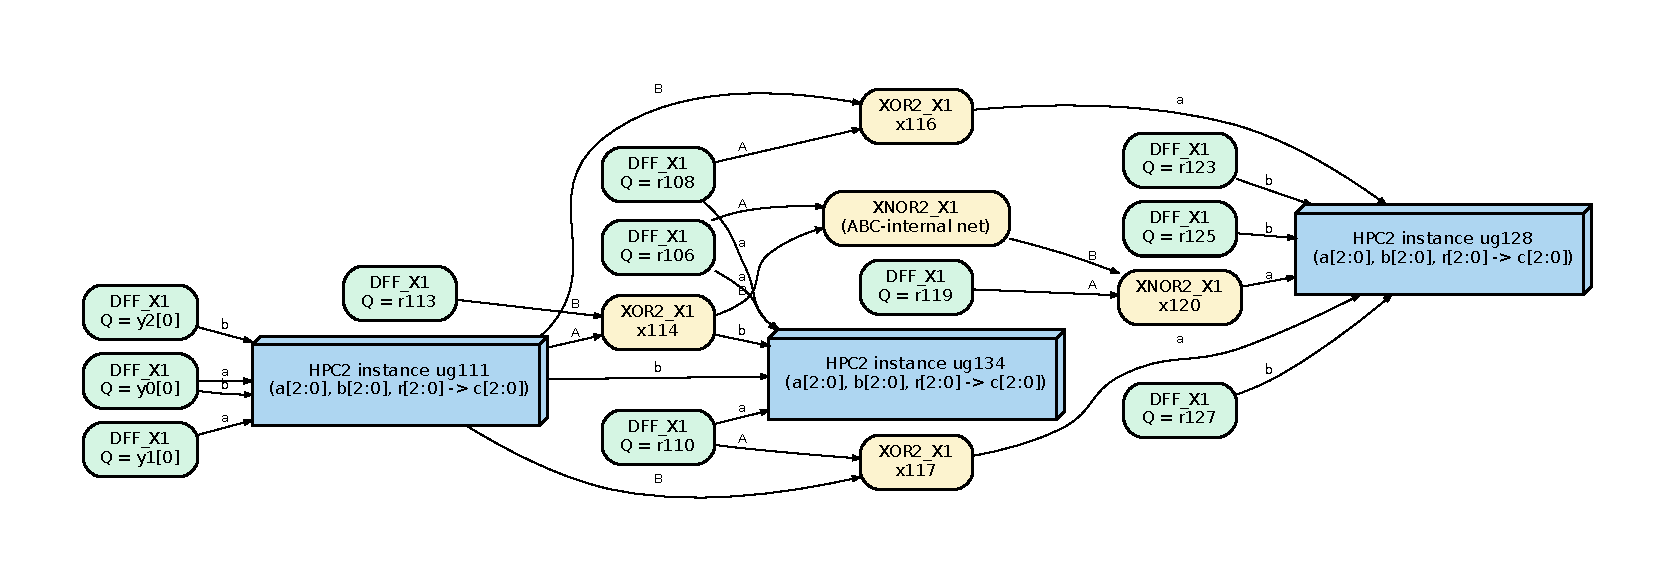
\includegraphics[width=0.9\textwidth]{figures/gates/slice_bit1.pdf}
\caption{Real mapped subcircuit around the bit-1 gadgets of \sig{pams\_jqr}, automatically extracted from \file{competitors/runs/syn\_pams\_jqr\_p0/mapped.json} (Yosys flow B, mapping 0) and drawn with Graphviz.
\textbf{Gadgets:} \sig{ug111} (CSA majority, bit 0), \sig{ug134} (carry $c_2$) and \sig{ug128} (comparator step $\lt_2$).
\textbf{Other cells:} green = \sig{DFF\_X1} (Q net named), yellow = combinational cells.
\textbf{Edges:} solid = into gadget port \sig{a} or cell input \sig{A}; dashed = into gadget port \sig{b} or cell input \sig{B}.}\label{fig:slice}
\end{figure*}

\paragraph{Physical level.}
\Cref{fig:placement} draws every placed standard cell of the routed reference runs (target 1.2\ns, seed 1, utilization 50\,\%), from OpenROAD's final DEF, at the same scale for both designs. Cells are classified by instance hierarchy and master cell.
\begin{itemize}
  \item \textbf{Gadgets (blue).} They occupy $7{,}242\um$ in \PAMS{} and $10{,}329\um$ in the baseline. This includes the hold buffers and tie cells OpenROAD inserted inside gadget hierarchies.
  \item \textbf{Pipeline and alignment flip-flops (green):} $5{,}851$ vs.\ $6{,}783\um$.
  \item \textbf{Other logic (orange):} mostly the share-wise multipliers, which cluster near the input pins; $3{,}906$ vs.\ $3{,}870\um$.
  \item \textbf{Buffers (grey):} $1{,}655$ vs.\ $2{,}199\um$.
  \item \textbf{Critical path (black).} The worst setup path of each design lies inside a share-wise multiplier stage: \sig{x1r[5]}$\to$\sig{ml1[23]} in \PAMS{} and \sig{x0r[9]}$\to$\sig{mh0[31]} in the baseline (\cref{fig:critpath}).
\end{itemize}
The OpenROAD-rendered routed layouts of the same runs are in \cref{app:physical}.

\begin{figure*}[t]\centering
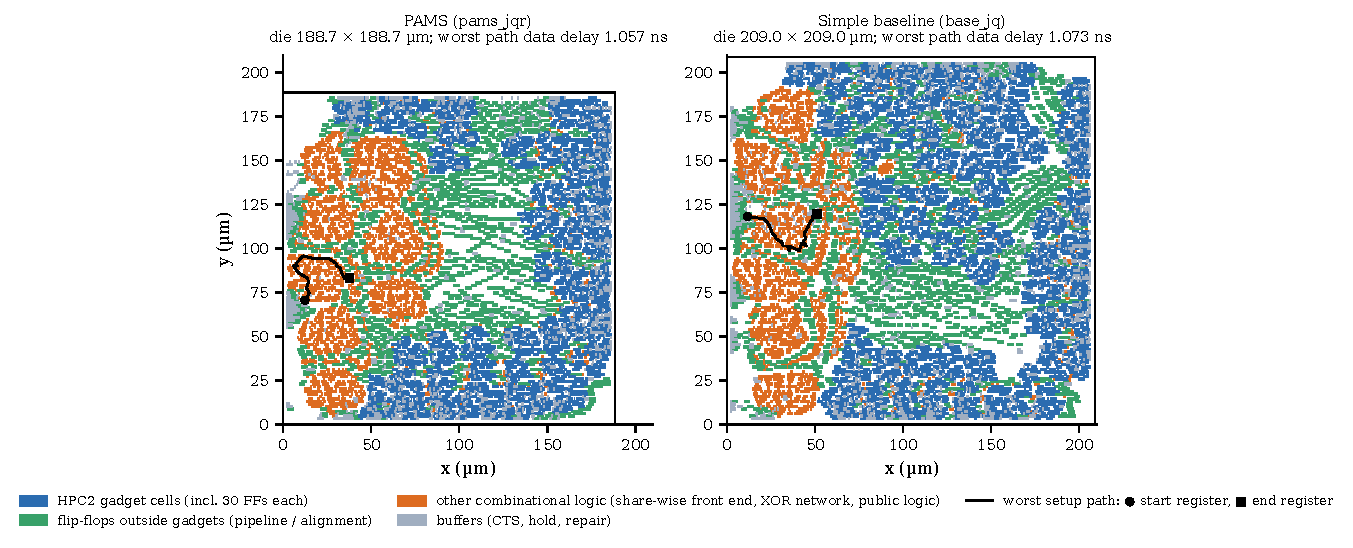
\includegraphics[width=\textwidth]{figures/physical/fig_placement.pdf}
\caption{Placed standard cells of the routed reference runs (target 1.2\ns, seed 1), drawn from the OpenROAD DEF files at equal scale. Tap and filler cells are omitted. The black polyline connects the cells of the worst setup path from \file{timing.rpt} (\cref{fig:critpath}). \PAMS{} fits in a $188.7 \times 188.7\,\si{\micro\meter}$ die; the baseline needs $209.0 \times 209.0\,\si{\micro\meter}$ at the same 50\,\% utilization.}\label{fig:placement}
\end{figure*}
